\section{从函数拟合开始}
% 引入拟合的基本思想
\subsection{最简单的规律——简单线性回归}

\begin{figure}[H]
    \centering
    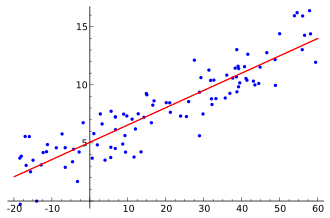
\includegraphics[width=0.6\textwidth]{img/linear_regression.png}
    \caption{线性回归示意图}
    {图源: \uhref{https://en.wikipedia.org/wiki/Linear_regression}{Wikipedia}}
    \label{fig:linear_regression}
\end{figure}

虽然\textoverset{Linear Regression}{线性回归}的名字叫做“\textoverset{Regression}{回归}”,但是事实上我更喜欢叫做\textoverset{Linear Fitting}{线性拟合}。它的目的是找到一条直线尽可能“贴近”数据点。在这一基础上,我们可以发现数据之间的规律,从而做出一些预测。不过这里有几个问题:
\begin{itemize}
    \item 为什么要用直线?为什么不用曲线?
    \item 为什么要用直线拟合数据点?这有什么用?
    \item “贴近”数据点的标准是什么?为什么要选择这个标准?
\end{itemize}

我认为用直线的原因无非两点:一是直线 $y = kx+b$ 简单且意义明确,又能处理不少的问题。几何上直线作为基本对象,尺子就能画出;代数上只需要加减乘除,一次函数我们也很早就学过了。而它的思想一路贯穿到了微积分的导数并延申到了线性代数。二是许多曲线的回归可以转为线性回归(见后文)。例如指数型的 $y = k \mathrm{e}^{\alpha x}$ 取对数变为 $z = \alpha x + \ln k$,又如分式型的 $y = (\alpha x + \beta)^{-1}$ 取倒数转化为 $z = \alpha x + \beta$,从而归结为线性拟合。因此带着线性拟合经验再去考虑曲线会更轻松。

至于其意义:一是找到数据的规律,二是做出预测。拟合的系数可以用于测算数据之间的关系,斜率 $k$ 表明输出对输入的敏感程度。一个经典例子是广告投放的\textoverset{Marginal Benefit}{边际效益}\footnote{边际效益:经济学概念,每增加单位投入,产出会增加多少单位},在一定范围内拟合收益与投入的关系,可以估算当前的边际效益,从而决定是否继续投放。而物理上,比值定义法定义的各种物理量,如电阻、电容等,最常用的测算方式都是线性拟合。例如测量电源输出的若干组电压和电流数据,并拟合出直线,斜率的绝对值是电源的内阻,同时截距顺带给出了电源的电动势,这样测得的数据就可以用于预测电源的输出情况。对我们所处的世界有定量的认识是科学的基础。可测量的数据和数学模型来描述、解释和预测自然现象是科学的基本方法,也是拟合的根本目的。

既然有了基本思路,那么如何选择“贴近”的标准呢?直接去度量一堆散点和直线的接近程度多少有点霰弹枪\footnote{霰弹枪:一种枪,射出的子弹像雨点一样散开}打移动靶的感觉,但是我们总是可以计算子弹打到了几环。换言之,两个相差的部分才是关键的,\textoverset{Residual}{\textbf{残差}}的概念由此产生。取出每个点实际值和拟合值的差,就得到了这样一个列表\footnote{记号说明:对于变量,无论是一维变量还是多维变量,一律采用斜体。对于具体的数据点,视是否为向量决定使用黑体还是斜体。例如 $r = y - \hat y$ 表示的是方程,所以全部采用斜体。但是具体数据的残差计算,例如 $\bfr = \bfy - \hat \bfy$,是对数据点的向量运算,所以采用正体。}(其中根据拟合函数 $\hat y_i = kx_i + b$ 计算出预测值):
\[
    \bfr = [r_1, r_2, \ldots, r_n] = [y_1 - \hat y_1, y_2 - \hat y_2, \ldots, y_n - \hat y_n]
\]

度量数据点与直线间偏差这一问题就转为了度量残差与 0 的偏差。还记得勾股定理吗?直角坐标系内一点到 0 的距离是坐标平方和的平方根,只不过这里残差列表是个 $n$ 维的向量,度量它偏离原点的程度就是向量的\textoverset{Norm}{模}。这个模越小,说明拟合的效果越好。这样我们就自然地引入了度量拟合效果的量化标准,不过实际应用中出于方便(特别是计算上的方便),通常省去开根号的一步,直接采用残差的平方和,此外还会除以样本点数得到“平均”的残差平方。习惯上称之为\textoverset{Mean Squared Error}{\textbf{均方误差}}(MSE):
\[
    \text{MSE} = \frac1n |\bfr|^2 = \frac1n \sum_{i=1}^n r_i^2
\]

在踏出下一步之前,我想这里有一点点思考的空间。例如:
\begin{itemize}
    \item 为什么要用平方和而不是直接相加呢?

          这是因为直接相加会有正负相互抵消的可能,度量出的偏差为 0 甚至为负实在是不合理,因此至少要保证每一项都是正数。但是这又引出下一个问题。

    \item 为什么不用绝对值呢?绝对值也是正的啊。

          从正态分布的角度看,选用平方和自有它的\uhref{https://www.zhihu.com/question/20447622/answer/25186207}{道理}。但是即使读者并不熟悉这些统计的背景,也可以从另一个角度理解:平方和的确是一个更好的度量方式,因为它对大的偏差更加敏感。例如一个残差为 2 的点和一个残差为 4 的点,直接绝对值相加的话是 6,在这里残差为 4 的点贡献了 $4 / 6 \approx 66.7\%$ 的偏差。而它们的平方和是 $2^2 + 4^2 = 20$,残差为 4 的点贡献提升到了 $4^2 / 20 = 80\%$,更加凸显出了 4 的偏差,反映了我们更“关注”这一大偏差的想法,更符合通常对“偏差”的直观认识。

    \item 为什么要除以样本点数 $n$ 呢?

          一方面是为了跨数据集比较,数据集的大小通常有区别,就像买东西的重量。这正如不能光看价格不看质量就评价 5 元 2 斤的苹果贵还是 3 元 1 斤的苹果贵,因此需要一个“单位”来衡量。另一方面,看完下一个问题你就会明白其中的精妙之处。

    \item 这里直接把所有的残差平方加了起来,但如果有的点重要一些怎么办?

          先说明一下这样的需求并非空想,有时测量条件决定了不同点的可靠性并不相同。以一个精度 1\% 的表为例,测量得到 1.00, 2.00, 3.00 时它们本身允许的误差分别是 0.01, 0.02, 0.03,而非相同。也就是说我们会觉得 1.00 的测量值从残差的大小上\footnote{残差的大小:严谨的说称作\textoverset{Absolute Error}{绝对误差}}更为可靠,这时似乎应该衡量一下点的“重要性”。如果你想说一个点很重要怎么办?直观上来讲你可能会想把它重复几遍,例如如果你很关心 $r_1$,你可能会想,这还不简单吗?在误差列表中把 $r_1$ 重复 3 遍就好,就像这样:
          \[
              \text{Refined }\bfr = [r_1, r_1, r_1, r_2, r_3, \ldots, r_n]
          \]

          这时再计算均方误差呢,变成了 $n+2$ 个点,一种我们设想的“\textoverset{Refined}{改善的}”均方误差公式就变成了这样:
          \[
              \text{Refined MSE} = \frac1{n+2} \left(2r_1^2 + \sum_{i=1}^{n+2} r_i^2\right)
          \]

          只不过这样的方式无疑有点“笨重”,再仔细想想呢?如果把 $1/(n+2)$ 乘到每一项上,就像这样:
          \[
              \text{Refined MSE} = \frac3{n+2} r_1^2 + \frac1{n+2} r_2^2 + \cdots + \frac1{n+2} r_{n+2}^2
          \]

          再对照着上面的列表看一看,$3/(n+2)$ 不正好表明在大小为 $n+2$ 的列表中 $r_1$ 出现了 3 此吗?频次就这样和\textoverset{Weight}{权重}(系数)联系起来了。我们也没必要守着重复 3 次或者 5 次这种固定的规则——至少自然可没有限制重要性之间的比例刚好是整数。这样一来只需要一个权重列表就可以了,权重乘在残差平方前,这就引出了\textoverset{Weighted Error}{\textbf{加权误差}},大权重表示更重要,略微改写一下公式得到:
          \[
              \text{Weighted MSE} = \sum_{i=1}^n w_i r_i^2
          \]

          这里为了方便起见,假设了权重的和为 1,即 $\sum_{i=1}^n w_i = 1$,如果不为 1,可以先计算误差再除以权重的和。由此可以根据实际情况调整不同点的重要性,也可以看出,之前的均方误差不过是因为在 $n$ 个数中每个残差变量都出现了 1 次,所以权重都设为了 $1/n$。在重要性可变时,加权均方误差无疑提供了一种更加“通用”的\textoverset{Measurement Metrics}{度量方式}。
\end{itemize}

使用的工具已经准备好了,目标也已经明确了,那么可以开始拟合了。当然,为了简单起见,这里还是只考虑无权重的情况。我们要做的是找到一组\textoverset{Optimal}{最优的}\textoverset{Parameter}{参数值} $\hat k, \hat b$ 使得均方误差最小,从这一点可以窥见贯穿整个机器学习的核心思想——\textoverset{Minimize}{最小化}\textoverset{Loss}{损失}(误差)。形式上,公式会这么写:
\[
    \hat k, \hat b = \argmin_{k, b} \text{MSE} = \argmin_{k, b} \frac1n \sum_{i=1}^n (y_i - kx_i - b)^2
\]

但是它并没有那么神秘:$\arg$ 是 argument 的缩写\footnote{Argument: 自变量,数学优化中函数的输入变量。然而 $\argmin$ 中的 $\arg$ 仅仅表明在优化算法看来 $k, b$ 是可变的、待优化的自变量。但是从拟合模型外看过去,它们是固定的参变量,通常意义上仍称作 Parameter。这里 Argument 与 Parameter 的区别一定程度上体现了视角的转换。},$\min$ 则是 minimize 的缩写。上面的式子完全可以读作“\textoverset{Find the parameter values $k, b$ that minimize the MSE}{找到参数值 $\hat k, \hat b$ 使得均方误差最小}”。虽然项很多,但这本是上只是一个二次函数,所以无论是配方法、对 $k, b$ 分别求导还是使用矩阵方法,都可以很容易地求解。不过我很喜欢另一个较少被人提及的视角——从线性代数和几何的角度来看待这个问题。我们回头看看残差的表达式:
\[
    \begin{aligned}
        \bfr & = [r_1, r_2, \ldots, r_n]                                                     \\
          & = [y_1 - (kx_1 + b), y_2 - (kx_2 + b), \ldots, y_n - (kx_n + b)]              \\
          & = [y_1, y_2, \ldots, y_n] - (k [x_1, x_2, \ldots, x_n] + b [1, 1, \ldots, 1]) \\
    \end{aligned}
\]

我们暂时用一个这样的记号,记拟合所用的函数在这些数据点上的取值
\[
\begin{aligned}
    \bfx^0 &= [1, 1, \ldots, 1]\\
    \bfx^1 &= [x_1, x_2, \ldots, x_n]\\
\end{aligned}
\]
并记输出 $\bfy = [y_1, y_2, \ldots, y_n]$,那么残差就可以写成 $\bfr = \bfy - (k\bfx^1 + b\bfx^0)$。这样一来,我们的目标是找到 $k, b$ 使得 $\bfr$ 的模最小。写到这里,从代数上看可能依然不够直观,让我们换个角度看看。

\begin{figure}[H]
    \centering
    \begin{tikzpicture}[>=Stealth, scale=1.5]
        \begin{axis}[
                view={-15}{20},      % 设置视角 (方位角, 俯仰角)
                axis lines=center,  % 轴从原点开始
                enlargelimits=false,
                ticks=none,         % 取消刻度
                colormap/viridis,
                axis line style={draw=gray},
                % xlabel={$x$},
                % ylabel={$y$},
                % zlabel={$z$}
            ]

            \coordinate (O) at (axis cs:0,0,0);
            \coordinate (Y) at (axis cs:-0.25, 0.6, 0.85);
            \coordinate (A) at (axis cs:-0.15, 0.4, 0.95);

            \addplot3[thick, ->] coordinates {(0,0,0) (1,1,1)} ;
            \node[above, scale=0.7] at (axis cs:1,1,1) {$\bfx^0$};

            \addplot3[thick, ->] coordinates {(0,0,0) (-1,0,1)};
            \node[left, scale=0.7] at (axis cs:-1,0,1) {$\bfx^1$};

            \addplot3[thin, purple!50, ->] coordinates {(0,0,0) (-0.25, 0.6, 0.85)};
            \node[left, purple!50, scale=0.7] at (Y) {$\bfy$};

            \addplot3[thin, blue!50, ->] coordinates {(0,0,0) (-0.15, 0.4, 0.95)};
            \node[right, blue!50, scale=0.7] at (A) {$k\bfx^1 + b\bfx^0$};

            \addplot3[red, dash pattern=on 0.5pt off 0.5pt, ->] coordinates {(-0.15,0.4,0.95) (-0.25, 0.6, 0.85)};
            \node[red, above, scale=0.7] at (axis cs:-0.2, 0.5, 0.9) {$\bfr$};

            \addplot3[thin, dash pattern=on 0.5pt off 0.5pt] coordinates {(0.4, 0.4, 0.4) (-0.15, 0.4, 0.95) (-0.55, 0, 0.55)};

            \addplot3[surf, color=blue!30, fill=blue!30, shader=flat, opacity=0.5]
            coordinates {(0,1,2) (1,1,1) (0,0,0) (-1,0,1) (0,1,2)};
        \end{axis}
    \end{tikzpicture}
    \caption{从几何的角度看残差}
\end{figure}

从几何上,$k\bfx^1 + b\bfx^0$ 落在 $\bfx^0$ 与 $\bfx^1$ 确定的平面上,求 $\bfr = \bfy - (k\bfx^1 + b\bfx^0)$ 的最小值实际上就是从点向平面做垂线并求垂线长。平面上的点恰好表示了那些可以精准拟合的数据,而偏离平面的部分则暗示了无论怎么用直线拟合都会有误差。不得不说从几何上看确实清晰很多,事实上也有人从几何角度给出了\uhref{https://www.bilibili.com/video/BV15zPBevERL}{推导},不过掠过这些细节,仅保留一个直观的印象也无大碍。本节的几篇推荐阅读中都用不同的方法解答了如何最小化误差,有详细的推导,因此这里不再赘述。但是我认为如果读者有一些基础的统计知识而且想记住线性回归推导出的结果,那么结论值得一提,不过跳过也无妨。计算出来的结论是这样的:

首先要计算的是样本中心点,对 $b$ 的导数项为 0 推出最优的直线必然经过样本中心点 $(\bar x, \bar y)$,其中
\[
    \bar x = \frac1n \sum_{i=1}^n x_i, \bar y = \frac1n \sum_{i=1}^n y_i
\]

即\textoverset{Mean}{均值}。

看斜率之前先看看\textoverset{Variance}{方差}和\textoverset{Covariance}{协方差},方差\footnote{此注释写给学过数理统计的读者:此处并非\textoverset{Sample Variance}{样本方差},样本方差除以的是 $n-1$}的表达式是
\[
    \text{Var}(\bfx) = \frac1n \sum_{i=1}^n (x_i - \bar x)^2
\]

是不是感觉很熟悉?这不就是自变量相对均值的 MSE 吗?而协方差的表达式是
\[
    \text{Cov}(\bfx, \bfy) = \frac1n \sum_{i=1}^n (x_i - \bar x)(y_i - \bar y)
\]

它把方差中的平方项换成了 $x$ 和 $x$ 的\textoverset{Cross Term}{交叉项},并由此体现出了\textoverset{Correlation}{相关关系}。接下来计算的是斜率 $k$,它的表达式是
\[
    \hat k = \frac{\sum_{i=1}^n (x_i - \bar x)(y_i - \bar y)}{\sum_{i=1}^n (x_i - \bar x)^2}
\]

虽然分子分母都是求和式,看起来有些复杂,但是总结起来其实就是协方差除以自变量的方差,即 $k = \text{Cov}(\bfx, \bfy) / \text{Var}(\bfx)$,如果把协方差看作一种乘法\footnote{此注释写给熟悉线性代数的同学:在\uhref{https://en.wikipedia.org/wiki/Inner_product_space\#Random_variables}{向量空间内积}的意义上这几乎正确},那么 $k = (\bfx\cdot \bfy) / (\bfx\cdot \bfx)$ 看起来确实挺像那么回事的。

这样一来,通过点-斜率式方程就可以得到最优的直线,那么直线拟合就告一段落了。

\begin{tcolorbox}[myrecommendbox, title=推荐阅读, breakable=false]
    \begin{itemize}
        \item 如果你想了解“回归”与“\textoverset{Least Squares}{最小二乘}”的含义:\\
              \textit{用人话讲明白线性回归Linear Regression - 化简可得的文章 - 知乎}\\
              \url{https://zhuanlan.zhihu.com/p/72513104}
        \item 如果你想阅读从求导法到线性代数方法的详尽公式推理:\\
              \textit{非常详细的线性回归原理讲解 - 小白Horace的文章 - 知乎}\\
              \url{https://zhuanlan.zhihu.com/p/488128941}
        \item 如果你想详细了解了线性回归中的术语、求解过程与几何诠释:\\
              \textit{机器学习| 算法笔记-线性回归(Linear Regression) - iamwhatiwant的文章 - 知乎}\\
              \url{https://zhuanlan.zhihu.com/p/139445419}
    \end{itemize}
\end{tcolorbox}

\newpage

\subsection{多项式拟合}

\begin{figure}[H]
    \centering
    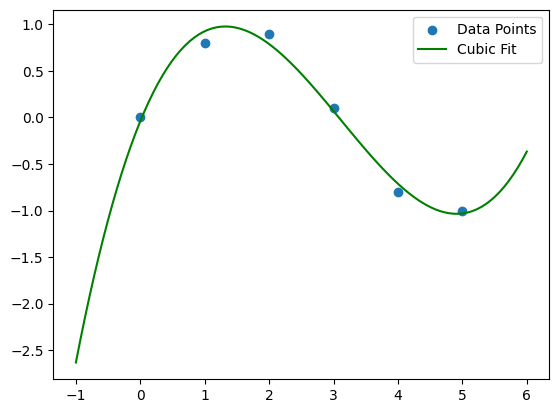
\includegraphics[width=0.6\textwidth]{img/polynomial_fitting.png}
    \caption{多项式拟合示意图(图为 3 次拟合)}
    {图源: \uhref{https://www.geeksforgeeks.org/numpys-polyfit-function-a-comprehensive-guide/}{GeeksforGeeks}}
    \label{fig:polynomial_fitting}
\end{figure}

线性拟合虽然很好,但是如果拿到了明显不线性的一堆数据,那么线性拟合就显得有些力不从心了。不过既然都是拟合,能做一次的那按理来讲也能做多次。\textoverset{Polynomial Fitting}{多项式拟合}就是这样一种思路,只是预测 $\hat y$ 从 $kx+b$ 变成了 $a_0 + a_1 x + \cdots + a_m x^m$\,\footnote{记号说明:虽然习惯上幂次从大到小排列,但是为了下标和幂次的统一性,所以这里选择从常数项到最高次项排列},其中 $m$ 是多项式的次数。而均方误差的表达式甚至几乎不用变,仍然是
\[
    \text{MSE} = \frac1n \sum_{i=1}^n (y_i - \hat y)^2
\]

只不过展开后是一系列的多项式项,待拟合的参数从两个变成了 $m+1$ 个。但是如果观察一下,这个式子仍然是一个(多变量的)二次函数,所以最小化的方法也是一样的。多项式自有多项式的好,能加的项多了,拟合的灵活性也就大了,误差显然会更小。然而与线性拟合相比,它虽然有\textoverset{Analytical Solution}{解析解},但不再像线性拟合一样可以逐项明确说出意义,而是只剩下一堆矩阵运算把这些参数算出来。因此相比于记下公式,形成一个整体上的印象显得尤为重要。

上一小节中,我们从图像看到了这种拟合的几何解释,而多项式拟合也是相似的,还是从 $\bfr$ 的表达式入手
\[
    \bfr = \bfy - (a_0 \bfx^0 + a_1 \bfx^1 + \cdots + a_m \bfx^m)
\]

对比之前的表达式,当 $a_0, a_1, \ldots, a_m$ 变化时,预测得到的结果 $\hat \bfy = a_0 \bfx^0 + a_1 \bfx^1 + \cdots + a_m \bfx^m$ 也会在一个 $m + 1$ 维的空间中变化,正如之前的平面,这个空间也是一个 $m + 1$ 维的子空间。求最小模的 $\bfr$ 又回到了从点到子空间的垂线问题。虽然不得不承认:想象从一个高维的 $n$ 维空间中向 $m+1$ 维的子空间做垂线确实有些困难,但是这多少离我们的几何直觉更近了一些。

系数的意义不那么明确了,但是误差下来了,这是好事吗?也不一定,灵活性的另一面是潜在的\textoverset{Overfitting}{\textbf{过拟合}}。前文中做线性拟合的时候有一个重要的假设是测量得到数据带有一定的误差。拟合的直线滤去了大部分的误差,留下了重要的趋势。但是如果灵活性太高,拟合的多项式会过于贴合数据,甚至把误差也拟合进去了。即使在给定的数据上做到了很小的误差,预测新数据的能力却可能会大打折扣。

拿做题打个比方:使用直线拟合明显不线性的数据是方法错了,只能说是没完全学会。但是用接近数据量的参数来拟合数据,留给它的空间都够把结果“背下来”了,捕捉到了数据的细节,却忽略了数据背后的规律,化成了一种只知道背答案的自我感动。在几道例题上能做到滴水不漏,但是一遇到新题就束手无策。

举个例子,在下面这个数据集上试图拟合,我们在二次函数 $y = 0.25 x^2 - x + 1$ 上添加了标准正态分布的噪声,即实际上 $y = 0.25 x^2 - x + 1 + \mathcal{N}(0, 1)$ \footnote{$\mathcal{N}(0, 1)$:表示一个服从\uhref{https://baike.baidu.com/item/\%E6\%A0\%87\%E5\%87\%86\%E6\%AD\%A3\%E6\%80\%81\%E5\%88\%86\%E5\%B8\%83}{标准正态分布}的变量,均值为 0,方差为 1}。
\newcommand{\drawrawdata}{
    \addplot[
        only marks,
        mark=*,
        color=blue
    ]
    coordinates {
            (0.0, 0.423) (0.1, -0.726) (0.2, 1.96) (0.3, 0.065) (0.4, -0.355) (0.5, 0.45) (0.6, -0.778) (0.7, 0.123) (0.8, 0.531) (0.9, -1.097) (1.0, 1.218) (1.1, -0.018) (1.2, 0.363) (1.3, -2.308) (1.4, -0.688) (1.5, 0.5) (1.6, 1.28) (1.7, -0.052) (1.8, 0.45) (1.9, -0.398) (2.0, 0.207) (2.1, 0.237) (2.2, -1.486) (2.3, 0.244) (2.4, -0.215) (2.5, -0.849) (2.6, 0.395) (2.7, -0.185) (2.8, -0.415) (2.9, -0.477) (3.0, 1.11) (3.1, -0.435) (3.2, 0.833) (3.3, 1.451) (3.4, 0.147) (3.5, 0.139) (3.6, -1.163) (3.7, 3.425) (3.8, -0.117) (3.9, 2.428) (4.0, 1.964) (4.1, 1.613) (4.2, 0.992) (4.3, 0.949) (4.4, 1.707) (4.5, 2.736) (4.6, 0.905) (4.7, 1.117) (4.8, 3.352) (4.9, 3.162) (5.0, 2.226) (5.1, 3.536) (5.2, 1.403) (5.3, 2.448) (5.4, 2.652) (5.5, 3.959) (5.6, 3.705) (5.7, 3.537) (5.8, 3.656) (5.9, 4.784) (6.0, 3.247) (6.1, 4.589) (6.2, 2.857) (6.3, 4.194) (6.4, 4.053) (6.5, 2.536) (6.6, 5.568) (6.7, 5.73) (6.8, 3.667) (6.9, 6.415) (7.0, 4.927) (7.1, 5.545) (7.2, 6.754) (7.3, 6.447) (7.4, 7.352) (7.5, 7.55) (7.6, 8.649) (7.7, 7.145) (7.8, 7.837) (7.9, 7.964) (8.0, 9.074) (8.1, 8.135) (8.2, 10.401) (8.3, 8.005) (8.4, 10.431) (8.5, 10.629) (8.6, 8.624) (8.7, 10.726) (8.8, 13.097) (8.9, 12.136) (9.0, 12.849) (9.1, 10.127) (9.2, 14.107) (9.3, 13.364) (9.4, 14.538) (9.5, 12.474) (9.6, 15.591) (9.7, 13.714) (9.8, 16.952) (9.9, 16.317) (10.0, 16.764)
        };
    \addlegendentry{带噪声数据}
}
\begin{figure}[h]
    \centering
    \begin{tikzpicture}
        \begin{axis}[
                axis lines=middle,
                xlabel={$x$}, ylabel={$y$},
                grid=major,
                legend pos=north west
            ]
            \drawrawdata
            \addplot[
                domain=0:10,
                samples=100,
                color=red,
                thick
            ] {0.25 * x^2 - x + 1};
            \addlegendentry{真实曲线}
        \end{axis}
    \end{tikzpicture}
\end{figure}

那么现在我们来试试用不同次数的多项式拟合这个数据集。不难看出线性拟合的线与数据点还是相差不少,因为它没能提供可以制造数据“弯曲”形状的项,2 次曲线的效果几乎和真实曲线一样,即使提升到 3 次也没有太明显的改变。
\begin{figure}[H]
    \centering
    \begin{tikzpicture}
        \begin{axis}[
                axis lines=middle,
                xlabel={$x$}, ylabel={$y$},
                grid=major,
                legend pos=north west
            ]
            \drawrawdata
            \addplot[
                domain=0:10,
                samples=100,
                color=red,
                thick
            ] {0.25 * x^2 - x + 1};
            \addlegendentry{真实曲线}

            \addplot[
                domain=0:10,
                samples=100,
                color=orange,
                thick
            ] {1.5142676761793825 * x -3.3366750145602806};
            \addlegendentry{线性拟合}

            \addplot[
                domain=0:10,
                samples=100,
                color=yellow,
                thick
            ] {0.24383409557403493 * x^2 -0.9240732795609664 * x + 0.6865875624112963};
            \addlegendentry{二次拟合}

            \addplot[
                domain=0:10,
                samples=100,
                color=green,
                thick
            ] {0.012628009463763832 * x^3 + 0.054413953617577414 * x^2 -0.17015585855533788 * x + 0.07400282332411103};
            \addlegendentry{三次拟合}
        \end{axis}
    \end{tikzpicture}
\end{figure}

但是如果继续增加次数呢?先来看看十次的拟合效果。
\begin{figure}[H]
    \centering
    \begin{tikzpicture}
        \begin{axis}[
                axis lines=middle,
                xlabel={$x$}, ylabel={$y$},
                grid=major,
                legend pos=north west
            ]
            \drawrawdata

            \addplot[
                domain=0:10,
                samples=100,
                color=red,
                thick
            ] {0.25 * x^2 - x + 1};
            \addlegendentry{真实曲线}

            \addplot[
                domain=0:10,
                samples=100,
                color=orange,
                thick
            ] {-0.000004129005667 * x^10 + 0.000200033877258 * x^9 - 0.004061827595427 * x^8 + 0.044810202155712 * x^7 - 0.291097682876070 * x^6 + 1.129425113256322 * x^5 - 2.542208192992861 * x^4 + 3.091776048493755 * x^3 - 1.584353162512058 * x^2 - 0.267618886184698 * x + 0.362912675589959};
            \addlegendentry{十次拟合}
        \end{axis}
    \end{tikzpicture}
\end{figure}

你可能会想,虽然是稍微歪了一点,不过这看起来还行吧。但是如果你把 $x$ 的范围稍微扩大一点,你就会发现势头完全不对了。
\begin{figure}[H]
    \centering
    \begin{tikzpicture}
        \begin{axis}[
                axis lines=middle,
                xlabel={$x$}, ylabel={$y$},
                grid=major,
                legend pos=south east
            ]
            \drawrawdata

            \addplot[
                domain=-1.5:11.5,
                samples=100,
                color=red,
                thick
            ] {0.25 * x^2 - x + 1};
            \addlegendentry{真实曲线}

            \addplot[
                domain=-1.5: 11.5,
                samples=100,
                color=orange,
                thick
            ] {(((((((((-0.000004129005667 * x + 0.000200033877258) * x - 0.004061827595427) * x + 0.044810202155712) * x - 0.291097682876070) * x + 1.129425113256322) * x - 2.542208192992861) * x + 3.091776048493755) * x - 1.584353162512058) * x - 0.267618886184698) * x + 0.362912675589959};
            \addlegendentry{十次拟合}
        \end{axis}
    \end{tikzpicture}
\end{figure}

一旦离开了拟合的区域,十次拟合的曲线就直勾勾地弯向无穷远,这是因为它把噪声也拟合进去了,从而给出了\textoverset{Generalization}{泛化性}\footnote{泛化性:预测原有数据集以外点的能力}极差的结果。这就是过拟合的危害。因为参数量与样本点数量并没有非常显著的差别(10 个参数,100 个样本点),所以从去噪声的角度看,结果过拟合并不奇怪——过滤掉噪声需要更多的数据。

当然解决办法并不是没有,要解决问题先要找到问题的根源。既然得到的函数行为不符合预期,那么很自然地我们会想问,这个函数的系数怎么样呢?在上面这个具体的例子中,函数的表达式是
\[
    \begin{aligned}
        \hat y & = -0.000004129005667 x^{10} + 0.000200033877258 x^9 - 0.004061827595427 x^8   \\
               & \quad + 0.044810202155712 x^7 - 0.291097682876070 x^6 + 1.129425113256322 x^5 \\
               & \quad - 2.542208192992861 x^4 + 3.091776048493755 x^3 - 1.584353162512058 x^2 \\
               & \quad - 0.267618886184698 x + 0.362912675589959
    \end{aligned}
\]

简单估算一下就会发现,例如 3, 4 次项的系数都在个位数级别,再乘以 $x$ 的 3 次方、4 次方数值就会变得很大。10 次方项的系数看起来只有 $4.1\times 10^{-6}$,但是乘上 $\bfx$ 中最大值的 10 次方,也就是 $10^{10}$ 后,这个数值同样会飙升到上万的级别。一堆上万级别的数加在一起,倒不如说顶着舍入误差\footnote{舍入误差:就像手动计算时保留几位小数一样,计算机计算的并不是“实数”,而是具有一定精度的浮点数,同样也有误差。例如对于 32-bit 的浮点数,只能精确到 7 个十进制位,这意味着从万位向后数到第 7 位,从百分位就可能已经不准确,在此之后的数位就不太可靠了。}还能够回归到原来的数据集上已经是奇迹了。也就只有 MSE 可以限制一下它在数据集内的行为,出了预定义的范围,这个高次函数大概就放飞自我了。

不过如果一定要用高次函数,补救的办法也不是没有。既然这些系数导致了很大的数值,那限制一下这些数值就好了,这就是\textoverset{Regularization}{\textbf{正则化}}的思路。我们在待优化的函数上加上一个\textoverset{Penalty Term}{惩罚项},同样地使用平方求和的形式,只不过这次是对系数进行惩罚,为了让系数尽量小,即尽量贴近于 $0$,自然想到把它们的平方也加起来(再乘以一个权重),优化的目标\footnote{Loss:损失,与前文单纯使用 MSE 时相同,我们希望让它尽可能小,它的每一项包含了我们对拟合结果的一个美好“祝愿”,MSE 项希望它误差减小,正则化项希望它系数正常。}变成了
\[
    \text{Loss} = \text{MSE} + \underset{\text{正则化项}}{\underbrace{\lambda \sum_{i=1}^{10} a_i^2}}
\]

可调参数 $\lambda$ 表明我们希望在多大程度上抑制系数。然而仍然有一个致命的问题:不同系数对最终结果的影响不同。例如在 $x=10$ 这一点上,$x^{10}$ 项的系数对结果的影响远远大于 $x$ 项的系数,即使是 $4.1\times 10^{-6}$ 这样微小的 $10$ 次项系数也会导致非常大的数值。平方后这一系数变得十分微小,原本用于约束系数大小的正则化项对它的影响更是微乎其微。那么怎么办呢?

再仔细想想问题在哪里,我们发现一路下来导致问题的根源都是 $x$ 的高次项即使在系数很小时也会导致数值爆炸。但是如果把 $x$ 放到 $[-1, 1]$ 的闭区间内呢?这样即使是 $x^{10}$ 项,$x$ 的 10 次方也不会超过 $1$,系数再怎么大,至少在小范围内也不会导致数值爆炸,这样一来正则化项才能发挥其约束作用。

操作上只需要把 $[0, 10]$ 范围内的 $x$ 线性地映射到 $[-1, 1]$ 范围内。这很简单,令 $z = 0.2 x - 1$ 再对 $y$ 用 $z$ 的多项式拟合,这种操作称作\textoverset{Normalization}{\textbf{归一化}}\footnote{归一化:调整数据到某个给定的范围内,使数据在不同场景下更加可比、更加数值稳定。前文计算误差时取平均实际上也是一种归一化。}。

事实上只需要一个很小的 $\lambda$ 就可以在一定程度上抑制高次项的系数,这里我们取 $\lambda = 0.01$,优化的目标变为了
\[
    \text{Loss} = \text{MSE} + 0.01 \sum_{i=1}^{10} a_i^2
\]

这时拟合出来的图像是这样的:

\begin{figure}[H]
    \centering
    \begin{tikzpicture}
        \begin{axis}[
                axis lines=middle,
                xlabel={$z$}, ylabel={$y$},
                grid=major,
                legend pos=north west
            ]

            \addplot[
                only marks,
                mark=*,
                color=blue
            ] coordinates {
                    (-1.0, 0.423) (-0.98, -0.726) (-0.96, 1.96) (-0.94, 0.065) (-0.92, -0.355) (-0.9, 0.45) (-0.88, -0.778) (-0.86, 0.123) (-0.84, 0.531) (-0.82, -1.097) (-0.8, 1.218) (-0.78, -0.018) (-0.76, 0.363) (-0.74, -2.308) (-0.72, -0.688) (-0.7, 0.5) (-0.68, 1.28) (-0.66, -0.052) (-0.64, 0.45) (-0.62, -0.398) (-0.6, 0.207) (-0.58, 0.237) (-0.56, -1.486) (-0.54, 0.244) (-0.52, -0.215) (-0.5, -0.849) (-0.48, 0.395) (-0.46, -0.185) (-0.44, -0.415) (-0.42, -0.477) (-0.4, 1.11) (-0.38, -0.435) (-0.36, 0.833) (-0.34, 1.451) (-0.32, 0.147) (-0.3, 0.139) (-0.28, -1.163) (-0.26, 3.425) (-0.24, -0.117) (-0.22, 2.428) (-0.2, 1.964) (-0.18, 1.613) (-0.16, 0.992) (-0.14, 0.949) (-0.12, 1.707) (-0.1, 2.736) (-0.08, 0.905) (-0.06, 1.117) (-0.04, 3.352) (-0.02, 3.162) (0.0, 2.226) (0.02, 3.536) (0.04, 1.403) (0.06, 2.448) (0.08, 2.652) (0.1, 3.959) (0.12, 3.705) (0.14, 3.537) (0.16, 3.656) (0.18, 4.784) (0.2, 3.247) (0.22, 4.589) (0.24, 2.857) (0.26, 4.194) (0.28, 4.053) (0.3, 2.536) (0.32, 5.568) (0.34, 5.73) (0.36, 3.667) (0.38, 6.415) (0.4, 4.927) (0.42, 5.545) (0.44, 6.754) (0.46, 6.447) (0.48, 7.352) (0.5, 7.55) (0.52, 8.649) (0.54, 7.145) (0.56, 7.837) (0.58, 7.964) (0.6, 9.074) (0.62, 8.135) (0.64, 10.401) (0.66, 8.005) (0.68, 10.431) (0.7, 10.629) (0.72, 8.624) (0.74, 10.726) (0.76, 13.097) (0.78, 12.136) (0.8, 12.849) (0.82, 10.127) (0.84, 14.107) (0.86, 13.364) (0.88, 14.538) (0.9, 12.474) (0.92, 15.591) (0.94, 13.714) (0.96, 16.952) (0.98, 16.317) (1.0, 16.764)
                };
            \addlegendentry{带噪声数据}

            \addplot[
                domain=-1.4: 1.4,
                samples=100,
                color=red,
                thick
            ] {0.25 * ((x+1)*5)^2 - (x+1)*5 + 1};
            \addlegendentry{真实曲线}

            \addplot[
                domain=-1.4:1.4,
                samples=100,
                color=orange,
                thick
            ] {0.056914714852145956 * x^10
                -0.16883868373880576 * x^9
                +0.2748227691835253 * x^8
                +0.02818103309527224 * x^7
                +0.8506420254328089 * x^6
                +0.5250028027489858 * x^5
                +1.8635063516688952 * x^4
                +1.8797071938317609 * x^3
                +3.414068726324771 * x^2
                +6.0490130644654645 * x^1
                +2.5048936484111635};
            \addlegendentry{十次拟合}
        \end{axis}
    \end{tikzpicture}
\end{figure}
\let\drawrawdata\relax

虽然图中拟合曲线与真值在数据集外确实仍然有显著的差距,但经过自变量归一化和参数正则化项的加入,拟合的曲线至少把数据的大体趋势成功地延伸到了数据集的一个邻域内,不至于像原本的那样惨不忍睹。

不过在实际应用中,几乎不会用到 5 次以上的多项式拟合。仍然是因为容易过拟合:就以 $[-1, 1]$ 上的函数为例,$x^5$ 与 $x^7$ 的图像几乎是一样的,它们最大的差值仅为 0.12,这意味着如果允许的高次项太多,一点点微小的噪声就能让轻易地把五次项的系数“分给”七次项,或者反之。这导致拟合的数值稳定性很差,因此显然不太可靠。从这种影响的角度看,高次多项式拟合本身就有\textoverset{Singularity}{奇异性},解并不稳定(这种对微小噪声敏感的问题常称为\textoverset{Ill-posed Problem}{病态问题})。因此比正则化或者归一化更重要的是,我们应该意识到高次函数并不是万能的。当你觉得需要用到很高次的函数才能成功拟合时,不如先想想,多项式的假设真的合适吗?

我们注意到一个重要的事实:虽然拟合的参数在变化,但是拟合前仍然需要人为地设定多项式的次数,正则项(如果有的话)权重也需要人为设定。这些\textoverset{Prior}{先验}的\footnote{先验:在观测到数据之前,我们已经了解了一些数据特征。}参数通常称为\textoverset{Hyperparameter}{\textbf{超参数}}。如何用模型拟合固然是重要的问题,但是模型的结构,包括如何选取适当的超参数也有学问。因为它们通常不是直接从数据中学习的,而需要人为设定。\uhref{https://www.zhihu.com/question/625846838/answer/3251736042}{有道是}“学而不思则\textoverset{Underfitting}{欠拟合},思而不学则过拟合”,我们只有在一定程度上了解问题的本质才能做出适当的选择。

\begin{tcolorbox}[myrecommendbox, title=推荐阅读, breakable=false]
    \begin{itemize}
        \item 如果你想看更多关于多项式拟合的实战,可以阅读:\\
              \textit{多项式拟合的介绍与例子 - 姓甚名谁的文章 - 知乎}\\
              \url{https://zhuanlan.zhihu.com/p/366870301}
        \item 如果你曾经想过拿问卷调查来做拟合,可以看看:\\
              \textit{理科生觉得哪些知识不知道是文科生的遗憾? - 一只小猫咪的回答 - 知乎}\\
              \url{https://www.zhihu.com/question/270455074/answer/2374983755}
        \item 这个比喻很好,同一问题下的其它回答也很有趣:\\
              \textit{人的大脑会不会出现“过拟合”病? - 莲梅莉usamimeri的回答 - 知乎}\\
              \url{https://www.zhihu.com/question/625846838/answer/3250463511}
    \end{itemize}
\end{tcolorbox}

\newpage

\subsection{高维的线性拟合}

\begin{figure}[H]
    \centering
    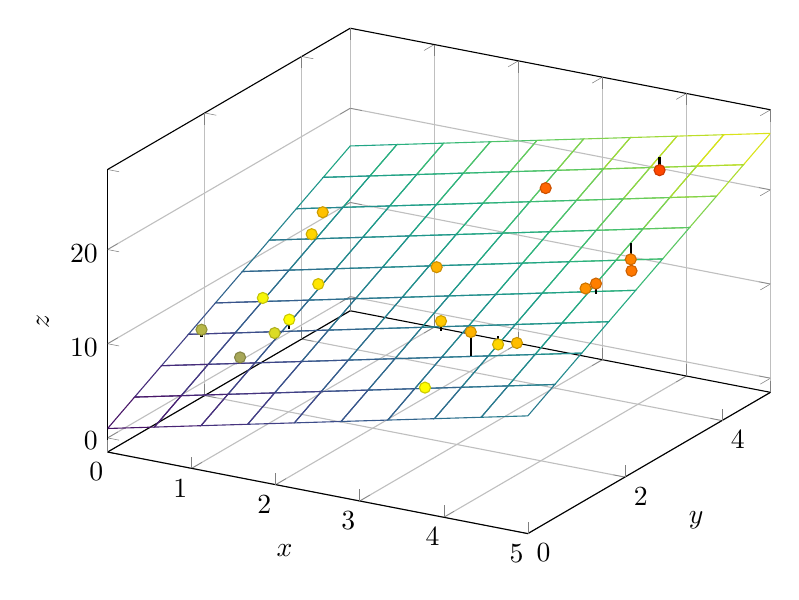
\begin{tikzpicture}
        \begin{axis}[
                view={30}{30}, % 3D视角
                xlabel={$x$}, % x轴标签
                ylabel={$y$}, % y轴标签
                zlabel={$z$}, % z轴标签
                grid=both, % 显示网格
                width=10cm, % 图形宽度
                height=8cm, % 图形高度
            ]

            % 绘制三维回归曲面
            \addplot3[
                mesh,
                domain=0:5,
                y domain=0:5,
                samples=10, % 控制采样的精细度
                colormap/viridis % 曲面的颜色映射
            ]
            {2*x + 3*y + 1}; % 这是回归方程 z = 2x + 3y + 1

            % 绘制数据点
            \addplot3[
                only marks,
                scatter,
                mark=*, % 点的形状
                red
            ] coordinates {
                    (3.795, 1.474, 12.073)
                    (1.06, 1.606, 8.15)
                    (4.727, 2.609, 18.101)
                    (3.045, 1.597, 12.882)
                    (2.382, 2.655, 14.288)
                    (2.869, 4.058, 19.319)
                    (4.354, 2.308, 16.486)
                    (4.556, 2.173, 17.759)
                    (3.427, 0.605, 9.461)
                    (0.542, 2.26, 9.017)
                    (0.187, 1.612, 6.976)
                    (1.109, 2.421, 10.991)
                    (3.897, 4.625, 21.301)
                    (0.437, 3.448, 12.044)
                    (3.68, 1.11, 14.286)
                    (0.387, 3.763, 13.343)
                    (1.171, 1.715, 9.446)
                    (0.881, 1.204, 6.461)
                    (4.165, 1.221, 13.633)
                    (4.448, 3.077, 17.432)
                };

            % 绘制数据点到平面竖直方向的连线
            \draw[black, thick] (axis cs:3.795,1.474,12.073) -- (axis cs:3.795,1.474,13.012);
            \draw[black, thick] (axis cs:1.06,1.606,8.15) -- (axis cs:1.06,1.606,7.938);
            \draw[black, thick] (axis cs:4.727,2.609,18.101) -- (axis cs:4.727,2.609,18.281);
            \draw[black, thick] (axis cs:3.045,1.597,12.882) -- (axis cs:3.045,1.597,11.881);
            \draw[black, thick] (axis cs:2.382,2.655,14.288) -- (axis cs:2.382,2.655,13.729);
            \draw[black, thick] (axis cs:2.869,4.058,19.319) -- (axis cs:2.869,4.058,18.912);
            \draw[black, thick] (axis cs:4.354,2.308,16.486) -- (axis cs:4.354,2.308,16.632);
            \draw[black, thick] (axis cs:4.556,2.173,17.759) -- (axis cs:4.556,2.173,16.631);
            \draw[black, thick] (axis cs:3.427,0.605,9.461) -- (axis cs:3.427,0.605,9.669);
            \draw[black, thick] (axis cs:0.542,2.26,9.017) -- (axis cs:0.542,2.26,8.864);
            \draw[black, thick] (axis cs:0.187,1.612,6.976) -- (axis cs:0.187,1.612,6.21);
            \draw[black, thick] (axis cs:1.109,2.421,10.991) -- (axis cs:1.109,2.421,10.481);
            \draw[black, thick] (axis cs:3.897,4.625,21.301) -- (axis cs:3.897,4.625,22.669);
            \draw[black, thick] (axis cs:0.437,3.448,12.044) -- (axis cs:0.437,3.448,12.218);
            \draw[black, thick] (axis cs:3.68,1.11,14.286) -- (axis cs:3.68,1.11,11.69);
            \draw[black, thick] (axis cs:0.387,3.763,13.343) -- (axis cs:0.387,3.763,13.063);
            \draw[black, thick] (axis cs:1.171,1.715,9.446) -- (axis cs:1.171,1.715,8.487);
            \draw[black, thick] (axis cs:0.881,1.204,6.461) -- (axis cs:0.881,1.204,6.374);
            \draw[black, thick] (axis cs:4.165,1.221,13.633) -- (axis cs:4.165,1.221,12.993);
            \draw[black, thick] (axis cs:4.448,3.077,17.432) -- (axis cs:4.448,3.077,19.127);
        \end{axis}
    \end{tikzpicture}
    \caption{高维线性拟合示例}
\end{figure}

第一节我们介绍了“简单线性回归”,即只有一个自变量的线性回归。但是在实际问题中,自变量往往不止一个,这时一元的线性回归就需要改成\textoverset{Multiple Linear Regression}{多元线性回归}。不过按照我的习惯,文中仍然称为“拟合”。

现实世界中的数据往往是多维的,就以估计体重为例,不难发现年龄和身高就是两个可能相关的变量。如果我们想用一个模型来描述这种相关性的话,最简单的就是线性模型了,与之前的 $\hat y=k x+b$ 类似,自然想到用这样的函数\footnote{记号说明:这里使用字母 $w$ 表示\textoverset{weight}{权重},$b$ 表示\textoverset{bias}{偏置},即常数项,$d$ 表示的是空间的\textoverset{dimension}{维度}。}去拟合数据:
\[
    \hat y = w_1 x_1 + w_2 x_2 + \cdots + w_d x_d + b
\]

同样地,优化的目标仍然是最小化均方误差,即对 $n$ 个数据点令
\[
    \text{MSE} = \frac{1}{n} \sum_{i=1}^{n} (y_i - \hat y_i)^2
\]

通过最小化误差得到 $w = [w_1, w_2, \cdots, w_d]$ 和 $b$ 的值。这个过程与一元线性回归的过程是类似的,只不过自变量是一维时,可以在平面上直接画出拟合的直线,二维时可以在空间中画出平面,但是当维数增加到三维及以上时,拟合所用的线性函数就变为\textoverset{Hyperplane}{超平面}了,我们无法直观地看到这个超平面,但是可以猜测,它的原理差不多。

话不多说,先看看效果。这里以美国人类学家 Richard McElreath 搜集到的一个年龄、身高与体重\uhref{https://github.com/rmcelreath/rethinking/blob/master/data/Howell1.csv}{数据集}为例,它的分布与拟合出来的平面是这样的:
\def\howelldata{
    (63.0, 151.765, 47.8256065) (63.0, 139.7, 36.4858065) (65.0, 136.525, 31.864838) (41.0, 156.845, 53.0419145) (51.0, 145.415, 41.276872) (35.0, 163.83, 62.992589) (32.0, 149.225, 38.2434755) (27.0, 168.91, 55.4799715) (19.0, 147.955, 34.869885) (54.0, 165.1, 54.487739) (47.0, 154.305, 49.89512) (66.0, 151.13, 41.220173) (73.0, 144.78, 36.0322145) (20.0, 149.9, 47.7) (65.3, 150.495, 33.849303) (36.0, 163.195, 48.5626935) (44.0, 157.48, 42.3258035) (31.0, 143.9418, 38.3568735) (12.0, 121.92, 19.617854) (8.0, 105.41, 13.947954) (6.5, 86.36, 10.489315) (39.0, 161.29, 48.987936) (29.0, 156.21, 42.7226965) (13.0, 129.54, 23.586784) (7.0, 109.22, 15.989118) (56.0, 146.4, 35.493574) (45.0, 148.59, 37.9032815) (19.0, 147.32, 35.4652245) (17.0, 137.16, 27.328918) (16.0, 125.73, 22.6796) (11.0, 114.3, 17.860185) (29.0, 147.955, 40.312989) (30.0, 161.925, 55.111428) (24.0, 146.05, 37.5063885) (35.0, 146.05, 38.498621) (33.0, 152.7048, 46.606578) (27.0, 142.875, 38.838815) (32.0, 142.875, 35.5786225) (36.0, 147.955, 47.400364) (24.0, 160.655, 47.8823055) (30.0, 151.765, 49.4131785) (24.0, 162.8648, 49.384829) (52.0, 171.45, 56.5572525) (42.0, 147.32, 39.12231) (19.0, 147.955, 49.89512) (17.0, 144.78, 28.803092) (8.0, 121.92, 20.41164) (12.0, 128.905, 23.359988) (5.0, 97.79, 13.267566) (55.0, 154.305, 41.2485225) (43.0, 143.51, 38.55532) (20.0, 146.7, 42.4) (18.0, 157.48, 44.6504625) (13.0, 127.0, 22.0105518) (9.0, 110.49, 15.422128) (5.0, 97.79, 12.757275) (42.0, 165.735, 58.5984165) (44.0, 152.4, 46.719976) (60.0, 141.605, 44.22522) (20.0, 158.8, 50.9) (37.0, 155.575, 54.317642) (50.0, 164.465, 45.8978405) (50.0, 151.765, 48.024053) (31.0, 161.29, 52.219779) (25.0, 154.305, 47.62716) (23.0, 145.415, 45.642695) (52.0, 145.415, 42.410852) (79.3, 152.4, 36.4858065) (35.0, 163.83, 55.9335635) (27.0, 144.145, 37.194544) (13.0, 129.54, 24.550667) (14.0, 129.54, 25.627948) (38.0, 153.67, 48.307548) (39.0, 142.875, 37.3362915) (12.0, 146.05, 29.596878) (30.0, 167.005, 47.173568) (24.0, 158.4198, 47.286966) (0.599999999999909, 91.44, 12.927372) (51.0, 165.735, 57.549485) (46.0, 149.86, 37.931631) (17.0, 147.955, 41.900561) (12.0, 137.795, 27.5840635) (22.0, 154.94, 47.2019175) (29.0, 160.9598, 43.204638) (38.0, 161.925, 50.2636635) (30.0, 147.955, 39.3774555) (6.0, 113.665, 17.463292) (45.0, 159.385, 50.689) (47.0, 148.59, 39.4341545) (79.0, 136.525, 36.28736) (45.0, 158.115, 46.266384) (54.0, 144.78, 42.2691045) (31.0, 156.845, 47.62716) (23.0, 179.07, 55.7067675) (9.0, 118.745, 18.824068) (41.0, 170.18, 48.5626935) (23.0, 146.05, 42.807745) (36.0, 147.32, 35.0683315) (5.0, 113.03, 17.8885345) (30.0, 162.56, 56.755699) (12.0, 133.985, 27.442316) (34.0, 152.4, 51.255896) (44.0, 160.02, 47.230267) (43.0, 149.86, 40.936678) (73.3, 142.875, 32.715323) (38.0, 167.005, 57.0675435) (43.0, 159.385, 42.977842) (33.0, 154.94, 39.9444455) (16.0, 148.59, 32.4601775) (11.0, 111.125, 17.123098) (6.0, 111.76, 16.499409) (35.0, 162.56, 45.9545395) (29.0, 152.4, 41.106775) (12.0, 124.46, 18.257078) (9.0, 111.76, 15.081934) (7.59999999999991, 86.36, 11.4815475) (58.0, 170.18, 47.5988105) (53.0, 146.05, 37.5063885) (51.0, 159.385, 45.019006) (48.0, 151.13, 42.2691045) (29.0, 160.655, 54.8562825) (41.0, 169.545, 53.523856) (81.75, 158.75, 52.1914295) (1.0, 74.295, 9.752228) (35.0, 149.86, 42.410852) (46.0, 153.035, 49.5832755) (5.0, 96.52, 13.097469) (29.0, 161.925, 41.730464) (42.0, 162.56, 56.018612) (27.0, 149.225, 42.1557065) (8.0, 116.84, 19.391058) (6.0, 100.076, 15.081934) (22.0, 163.195, 53.0986135) (43.0, 161.925, 50.235314) (53.0, 145.415, 42.52425) (43.0, 163.195, 49.101334) (41.0, 151.13, 38.498621) (50.0, 150.495, 49.8100715) (15.0, 141.605, 29.313383) (33.0, 170.815, 59.760746) (3.0, 91.44, 11.7083435) (62.0, 157.48, 47.9390045) (49.0, 152.4, 39.292407) (17.0, 149.225, 38.1300775) (12.0, 129.54, 21.999212) (22.0, 147.32, 36.8826995) (29.0, 145.415, 42.127357) (8.0, 121.92, 19.787951) (5.0, 113.665, 16.782904) (33.0, 157.48, 44.565414) (34.0, 154.305, 47.853956) (12.0, 120.65, 21.1770765) (7.0, 115.6, 18.9) (42.0, 167.005, 55.1964765) (40.0, 142.875, 32.998818) (27.0, 152.4, 40.879979) (3.0, 96.52, 13.267566) (25.0, 160.0, 51.2) (29.0, 159.385, 49.044635) (45.0, 149.86, 53.4388075) (26.0, 160.655, 54.090846) (45.0, 160.655, 55.3665735) (45.0, 149.225, 42.240755) (11.0, 125.095, 22.3677555) (85.5999999999999, 140.97, 40.936678) (26.0, 154.94, 49.6966735) (24.0, 141.605, 44.338618) (57.0, 160.02, 45.9545395) (22.0, 150.1648, 41.95726) (24.0, 155.575, 51.482692) (6.0, 103.505, 12.757275) (4.0, 94.615, 13.0124205) (21.0, 156.21, 44.111822) (79.0, 153.035, 32.205032) (50.0, 167.005, 56.755699) (40.0, 149.86, 52.673371) (64.0, 147.955, 36.4858065) (32.0, 159.385, 48.8461885) (38.7, 161.925, 56.9541455) (26.0, 155.575, 42.0990075) (63.0, 159.385, 50.178615) (62.0, 146.685, 46.549879) (22.0, 172.72, 61.80191) (41.0, 166.37, 48.987936) (19.0, 141.605, 31.524644) (17.0, 142.875, 32.205032) (14.0, 133.35, 23.756881) (9.0, 127.635, 24.4089195) (7.0, 119.38, 21.5172705) (74.0, 151.765, 35.2951275) (41.0, 156.845, 45.642695) (33.0, 148.59, 43.885026) (53.0, 157.48, 45.5576465) (18.0, 149.86, 39.008912) (37.0, 147.955, 41.163474) (6.0, 102.235, 13.1258185) (61.0, 153.035, 45.245802) (44.0, 160.655, 53.637254) (35.0, 149.225, 52.3048275) (7.0, 114.3, 18.3421265) (4.0, 100.965, 13.7495075) (23.0, 138.43, 39.0939605) (4.0, 91.44, 12.530479) (55.0, 162.56, 45.699394) (53.0, 149.225, 40.3980375) (59.0, 158.75, 51.482692) (57.0, 149.86, 38.668718) (35.0, 158.115, 39.235708) (29.0, 156.21, 44.338618) (62.0, 148.59, 39.519203) (18.0, 143.51, 31.071052) (51.0, 154.305, 46.776675) (14.0, 131.445, 22.509503) (19.0, 157.48, 40.6248335) (42.0, 157.48, 50.178615) (25.0, 154.305, 41.276872) (6.0, 107.95, 17.57669) (41.0, 168.275, 54.6) (37.0, 145.415, 44.9906565) (16.0, 147.955, 44.735511) (5.0, 100.965, 14.401546) (9.0, 113.03, 19.050864) (82.0, 149.225, 35.8054185) (28.0, 154.94, 45.2174525) (50.0, 162.56, 48.1091015) (43.0, 156.845, 45.6710445) (8.0, 123.19, 20.808533) (31.0, 161.0106, 48.420946) (67.0, 144.78, 41.1918235) (39.0, 143.51, 38.4135725) (18.0, 149.225, 42.127357) (11.0, 110.49, 17.6617385) (48.0, 149.86, 38.2434755) (30.0, 165.735, 48.3358975) (64.0, 144.145, 38.9238635) (72.0, 157.48, 40.029494) (68.0, 154.305, 50.2069645) (44.0, 163.83, 54.2892925) (43.0, 156.21, 45.6) (16.0, 153.67, 40.766581) (13.0, 134.62, 27.1304715) (34.0, 144.145, 39.4341545) (10.0, 114.3, 20.4966885) (62.0, 162.56, 43.204638) (44.0, 146.05, 31.864838) (11.0, 120.65, 20.8935815) (31.0, 154.94, 45.4442485) (29.0, 144.78, 38.045029) (8.0, 106.68, 15.989118) (62.0, 146.685, 36.0889135) (67.0, 152.4, 40.879979) (57.0, 163.83, 47.910655) (32.0, 165.735, 47.7122085) (24.0, 156.21, 46.379782) (77.0, 152.4, 41.163474) (62.0, 140.335, 36.5992045) (17.0, 158.115, 43.09124) (67.0, 163.195, 48.137451) (70.0, 151.13, 36.7126025) (37.0, 171.1198, 56.5572525) (58.0, 149.86, 38.6970675) (35.0, 163.83, 47.4854125) (30.0, 141.605, 36.2023115) (5.0, 93.98, 14.288148) (26.0, 149.225, 41.276872) (5.0, 105.41, 15.2236815) (21.0, 146.05, 44.7638605) (41.0, 161.29, 50.4337605) (46.0, 162.56, 55.281525) (49.0, 145.415, 37.931631) (15.0, 145.415, 35.493574) (28.0, 170.815, 58.456669) (12.0, 127.0, 21.488921) (83.0, 159.385, 44.4236665) (54.0, 159.4, 44.4) (54.0, 153.67, 44.565414) (68.0, 160.02, 44.622113) (68.0, 150.495, 40.483086) (56.0, 149.225, 44.0834725) (15.0, 127.0, 24.4089195) (57.0, 142.875, 34.416293) (22.0, 142.113, 32.772022) (40.0, 147.32, 35.947166) (19.0, 162.56, 49.5549) (41.0, 164.465, 53.183662) (75.9000000000001, 160.02, 37.081146) (73.9000000000001, 153.67, 40.5114355) (49.0, 167.005, 50.6038575) (26.0, 151.13, 43.9700745) (17.0, 147.955, 33.792604) (13.0, 125.3998, 21.375523) (8.0, 111.125, 16.669506) (88.0, 153.035, 49.89) (68.0, 139.065, 33.5941575) (33.0, 152.4, 43.8566765) (26.0, 154.94, 48.137451) (56.0, 147.955, 42.751046) (16.0, 143.51, 34.8415355) (13.0, 117.983, 24.097075) (34.0, 144.145, 33.906002) (5.0, 92.71, 12.076887) (17.0, 147.955, 41.276872) (74.0, 155.575, 39.7176495) (69.0, 150.495, 35.947166) (50.0, 155.575, 50.915702) (44.0, 154.305, 45.756093) (15.0, 130.6068, 25.2594045) (5.0, 101.6, 15.3370795) (18.0, 157.48, 49.214732) (41.0, 168.91, 58.8252125) (27.0, 150.495, 43.4597835) (8.90000000000009, 111.76, 17.8318355) (38.0, 160.02, 51.9646335) (57.0, 167.64, 50.688906) (64.5, 144.145, 34.246196) (42.0, 145.415, 39.3774555) (24.0, 160.02, 59.5622995) (16.0, 147.32, 40.312989) (71.0, 164.465, 52.16308) (49.5, 153.035, 39.972795) (33.0, 149.225, 43.941725) (28.0, 160.02, 54.601137) (47.0, 149.225, 45.075705) (3.0, 85.09, 11.453198) (1.0, 84.455, 11.7650425) (1.0, 59.6138, 5.896696) (3.0, 92.71, 12.1052365) (6.0, 111.125, 18.313777) (5.0, 90.805, 11.3681495) (27.0, 153.67, 41.333571) (5.0, 99.695, 16.2442635) (1.0, 62.484, 6.80388) (2.0, 81.915, 11.8784405) (2.0, 96.52, 14.968536) (1.0, 80.01, 9.865626) (55.0, 150.495, 41.900561) (83.4000000000001, 151.765, 42.524) (12.0, 140.6398, 28.859791) (2.0, 88.265, 12.7856245) (63.0, 158.115, 43.147939) (52.0, 149.225, 40.82328) (49.0, 151.765, 42.864444) (31.0, 154.94, 46.209685) (9.0, 123.825, 20.581737) (6.0, 104.14, 15.87572) (35.0, 161.29, 47.853956) (35.0, 148.59, 42.52425) (7.0, 97.155, 17.066399) (5.0, 93.345, 13.1825175) (24.0, 160.655, 48.5059945) (41.0, 157.48, 45.869491) (32.0, 167.005, 52.900167) (43.0, 157.48, 47.570461) (6.0, 91.44, 12.927372) (1.0, 60.452, 5.6699) (15.0, 137.16, 28.91649) (63.0, 152.4, 43.544832) (21.0, 152.4, 43.431434) (1.0, 81.28, 11.509897) (2.0, 109.22, 11.7083435) (1.0, 71.12, 7.540967) (3.0, 89.2048, 12.700576) (1.0, 67.31, 7.200773) (1.0, 85.09, 12.360382) (1.0, 69.85, 7.7961125) (55.0, 161.925, 53.2120115) (38.0, 152.4, 44.678812) (3.0, 88.9, 12.5588285) (3.0, 90.17, 12.700576) (1.0, 71.755, 7.37087) (1.0, 83.82, 9.2135875) (28.0, 159.385, 47.2019175) (16.0, 142.24, 28.632995) (36.0, 142.24, 31.6663915) (38.0, 168.91, 56.4438545) (12.0, 123.19, 20.014747) (1.0, 74.93, 8.50485) (1.0, 74.295, 8.3064035) (3.0, 90.805, 11.623295) (48.0, 160.02, 55.791816) (1.0, 67.945, 7.9662095) (15.0, 135.89, 27.21552) (45.0, 158.115, 47.4854125) (3.0, 85.09, 10.8011595) (3.0, 93.345, 14.004653) (38.0, 152.4, 45.1607535) (21.0, 155.575, 45.529297) (50.0, 154.305, 48.874538) (41.0, 156.845, 46.5782285) (13.0, 120.015, 20.128145) (8.0, 114.3, 18.14368) (3.0, 83.82, 10.9145575) (30.0, 156.21, 43.885026) (12.0, 137.16, 27.158821) (7.0, 114.3, 19.050864) (4.0, 93.98, 13.834556) (21.0, 168.275, 56.0469615) (38.0, 147.955, 40.086193) (15.0, 139.7, 26.5634815) (19.0, 157.48, 50.802304) (1.0, 76.2, 9.2135875) (1.0, 66.04, 7.5693165) (31.0, 160.7, 46.3) (8.0, 114.3, 19.4194075) (16.0, 146.05, 37.9032815) (21.0, 161.29, 49.3564795) (0.0, 69.85, 7.314171) (13.0, 133.985, 28.1510535) (0.0, 67.945, 7.824462) (50.0, 150.495, 44.111822) (39.0, 163.195, 51.0291) (44.0, 148.59, 40.766581) (36.0, 148.59, 37.5630875) (36.0, 161.925, 51.59609) (18.0, 153.67, 44.8205595) (0.0, 68.58, 8.0229085) (58.0, 151.13, 43.4030845) (58.0, 163.83, 46.719976) (33.0, 153.035, 39.5475525) (21.5, 151.765, 34.7848365) (11.0, 132.08, 22.792998) (26.0, 156.21, 39.292407) (22.0, 140.335, 37.4496895) (28.0, 158.75, 48.6760915) (42.0, 142.875, 35.606972) (2.0, 84.455, 9.3836845) (21.0, 151.9428, 43.714929) (19.0, 161.29, 48.19415) (13.0, 127.9906, 29.8520235) (48.0, 160.9852, 50.972401) (46.0, 144.78, 43.998424) (11.0, 132.08, 28.292801) (8.0, 117.983, 20.354941) (25.0, 160.02, 48.19415) (16.0, 154.94, 39.179009) (51.0, 160.9852, 46.6916265) (25.0, 165.989, 56.415505) (28.0, 157.988, 48.591043) (26.0, 154.94, 48.2224995) (5.0, 97.9932, 13.2959155) (1.0, 64.135, 6.6621325) (54.0, 160.655, 47.4854125) (66.0, 147.32, 35.550273) (20.0, 146.7, 36.6) (25.0, 147.32, 48.9595865) (38.0, 172.9994, 51.255896) (51.0, 158.115, 46.5215295) (48.0, 147.32, 36.967748) (13.0, 124.9934, 25.117657) (6.0, 106.045, 16.272613) (27.0, 165.989, 48.647742) (22.0, 149.86, 38.045029) (1.0, 76.2, 8.50485) (60.0, 161.925, 47.286966) (15.0, 140.0048, 28.3495) (0.0, 66.675, 8.1363065) (0.0, 62.865, 7.200773) (43.0, 163.83, 55.394923) (12.0, 147.955, 32.488527) (27.0, 160.02, 54.204244) (30.0, 154.94, 48.477645) (29.0, 152.4, 43.0628905) (0.0, 62.23, 7.257472) (23.0, 146.05, 34.189497) (30.0, 151.9936, 49.951819) (17.0, 157.48, 41.3052215) (0.0, 55.88, 4.8477645) (0.0, 60.96, 6.23689) (41.0, 151.765, 44.338618) (42.0, 144.78, 33.45241) (7.0, 118.11, 16.896302) (3.0, 78.105, 8.221355) (43.0, 160.655, 47.286966) (35.0, 151.13, 46.1246365) (10.0, 121.92, 20.184844) (3.0, 92.71, 12.757275) (75.5, 153.67, 47.400364) (64.0, 147.32, 40.8516295) (38.0, 139.7, 50.348712) (24.2, 157.48, 45.132404) (4.0, 91.44, 11.623295) (26.0, 154.94, 42.240755) (19.0, 143.51, 41.6454155) (2.0, 83.185, 9.1568885) (43.0, 158.115, 45.2174525) (38.0, 147.32, 51.255896) (10.0, 123.825, 21.205426) (3.0, 88.9, 11.5949455) (23.0, 160.02, 49.271431) (16.0, 137.16, 27.952607) (49.0, 165.1, 51.199197) (41.0, 154.94, 43.8566765) (6.0, 111.125, 17.690088) (23.0, 153.67, 35.5219235) (14.0, 145.415, 34.246196) (43.0, 141.605, 42.88542) (15.0, 144.78, 32.545226) (21.0, 163.83, 46.776675) (24.0, 161.29, 41.8722115) (20.0, 154.9, 38.2) (20.0, 161.3, 43.3) (34.0, 170.18, 53.637254) (29.0, 149.86, 42.977842) (11.0, 123.825, 21.54562) (3.0, 85.09, 11.4248485) (65.0, 160.655, 39.7743485) (46.0, 154.94, 43.3463855) (8.0, 106.045, 15.478827) (15.0, 126.365, 21.9141635) (43.0, 166.37, 52.673371) (39.0, 148.2852, 38.441922) (12.0, 124.46, 19.27766) (3.0, 89.535, 11.113004) (4.0, 101.6, 13.494362) (43.0, 151.765, 42.807745) (70.0, 148.59, 35.890467) (26.0, 153.67, 44.22522) (0.0, 53.975, 4.252425) (48.0, 146.685, 38.0733785) (0.0, 56.515, 5.159609) (5.0, 100.965, 14.3164975) (8.0, 121.92, 23.2182405) (3.0, 81.5848, 10.659412) (44.0, 154.94, 44.111822) (33.0, 156.21, 44.0267735) (15.0, 132.715, 24.9759095) (12.0, 125.095, 22.5945515) (5.0, 101.6, 14.344847) (41.0, 160.655, 47.8823055) (37.4, 146.05, 39.405805) (13.0, 132.715, 24.777463) (6.0, 87.63, 10.659412) (53.0, 156.21, 41.050076) (49.0, 152.4, 40.82328) (27.0, 162.56, 47.0318205) (7.0, 114.935, 17.519991) (1.0, 67.945, 7.2291225) (31.0, 142.875, 34.246196) (1.0, 76.835, 8.0229085) (17.0, 145.415, 31.127751) (31.0, 162.56, 52.16308) (21.0, 156.21, 54.0624965) (0.0, 71.12, 8.051258) (68.0, 158.75, 52.5316235)
                }
\begin{figure}[H]
    \centering
    \begin{tikzpicture}[>=Stealth, scale=1.5]
        \begin{axis}[
                view={120}{30}, % 3D视角
                xlabel={age}, % x轴标签
                ylabel={height}, % y轴标签
                zlabel={weight}, % z轴标签
                grid=both, % 显示网格
                width=10cm, % 图形宽度
                height=8cm, % 图形高度
            ]


            \addplot3[
                only marks,
                scatter,
                mark=*, % 点的形状
                red
            ] coordinates \howelldata;


            \addplot3[
                mesh,
                domain=0:90,
                y domain=50:180,
                samples=10, % 控制采样的精细度
                colormap/viridis % 曲面的颜色映射
            ]
            {0.04676645038926784*x + 0.47766688346191755*y - 31.805656676953056}; % 这是回归方程 z = 2x + 3y + 1

        \end{axis}
    \end{tikzpicture}
\end{figure}

通过拟合,我们可以得到一个超平面,它大致描述了数据的分布。这个超平面的方程是 $0.04676645038926784 \cdot \text{age} + 0.47766688346191755 \cdot \text{height} - 31.805656676953056 = \hat{\text{weight}}$,它比单纯使用身高或者年龄的拟合效果都要好一些。由此还可以量化地看到,年龄与身高都会影响体重,但是年龄是弱相关,而身高是强相关,这也符合我们的日常经验。

不过正如我们之前一直在做的一样,让我们看看更为直观的几何视角。仍然用 $\bfx^0$ 表示全 $1$ 的向量,使用 $\bfx_{:1}$ 表示所有样本的第一个\textoverset{Feature}{特征}(分量),$\bfx_{:2}$ 表示所有样本的第二个特征,以此类推\footnote{记号说明:冒号表示取所有行,这是为了与 Python 中 Numpy, Torch 等库的列切片语法 $a[:, j]$ 对齐。}。那么多元线性拟合时的残差向量变为了\footnote{记号说明:在公式中我特意将常数项放到了最前面,这是为了让它和多项式拟合的形式保持一致。}
\[
    \begin{aligned}
        \bfr = \bfy - \hat \bfy = \bfy - (b \bfx^0 + w_1 \bfx_{:1} + w_2 \bfx_{:2} + \cdots + w_d \bfx_{:d})
    \end{aligned}
\]

如果回顾一下我们在多项式拟合一节的内容,就会发现这和多项式时的残差向量
\[
    \bfr = \bfy - (a_0 \bfx^0 + a_1 \bfx^1 + a_2 \bfx^2 + \cdots + a_{m} \bfx^{m})
\]

有着惊人的相似之处。细心的读者可能已经发现,如果令这些分量 $\bfx_{:1}, \bfx_{:2}, \ldots, \bfx_{:n}$ 分别为 $\bfx$ 的幂次组成的向量 $\bfx^1, \bfx^2, \ldots, \bfx^d$,那么我们得到的完完全全就是多项式拟合。这也就意味着,多项式拟合实际上可以视为多元线性拟合的一种特殊情况。

事已至此,我们似乎已经许多次遇到了这样一种情况:从一面看过去,是代数上,一组样本点上的线性拟合。但是从另一面看过去,确是在几何上找到高维空间的超平面中最接近给定点的向量。这里其实有不少精妙的数学原理\footnote{写给数学基础好的读者:这本质上体现了代数与几何的\textoverset{Duality}{对偶性}。},但是考虑到这里的主题是机器学习,我将只带读者简要地复习(或者学习)一下线性代数,更为系统性地从几种略有差距的视角\footnote{
    几种视角:
    \textoverset{Overall}{整体}解读、
    \textoverset{Row-wise}{按行}解读、
    \textoverset{Column-wise}{按列}解读、
    \textoverset{Element-wise}{按元素}解读。
}体会矩阵的本质。

这里首先要感谢\uhref{https://github.com/kenjihiranabe/The-Art-of-Linear-Algebra}{The Art of Linear Algebra}这篇笔记,我初见就感到文中的插图画的非常精妙。它的思路是顺着 Gilbert Strang 教授书籍\uhref{https://math.mit.edu/~gs/everyone/}{Linear Algebra for Everyone}来的,我认为可以看成是一本矩阵图鉴,对理解矩阵运算有着极大的帮助。

\uhref{https://www.bilibili.com/video/BV1ys411472E}{3Blue1Brown 的线性代数系列}也是优质线性代数学习资源。这个制作精良的合集仅用不到两个小时的视频就清晰地从几何的角度讲明白了线性代数的基础知识,也是我入门线性代数的第一课。

矩阵有很多种\textoverset{Interpretation}{解读},不过我觉得大致可以按照是否把行看作一个整体以及是否把列看作一个整体来分为四类。
\begin{figure}[H]
    \centering
    \begin{tikzpicture}[>=Stealth]
        \pgfmathsetmacro{\elementsize}{0.7}
        \draw[<->] (-5, 0) node[above] {纵向切开}
        -- (5, 0) node[above] {把行视作整体};
        \draw[<->] (0, -5) node[below] {横向切开}
        -- (0, 5) node[above] {把列视作整体};
        \foreach \x in {-4, -3, -2, -1}{
                \foreach \y in {-4, -3, -2, -1}{
                        \fill [yellow] ({\x-\elementsize/2}, {\y-\elementsize/2}) rectangle ({\x+\elementsize/2}, {\y+\elementsize/2});
                    }
            }
        \foreach \x in {-4, -3, -2, -1}{
                \fill [green, opacity=0.5] ({\x-\elementsize/2}, {1-\elementsize/2}) rectangle ({\x+\elementsize/2}, {4+\elementsize/2});
            }
        \foreach \y in {-4, -3, -2, -1}{
                \fill [red, opacity=0.4] ({1-\elementsize/2}, {\y-\elementsize/2}) rectangle ({4+\elementsize/2}, {\y+\elementsize/2});
            }
        \fill [gray, opacity=0.5] ({1-\elementsize/2}, {1-\elementsize/2}) rectangle ({4+\elementsize/2}, {4+\elementsize/2});
        \node at (2.5, 2.5) {$f: \mathbb{R}^n \to \mathbb{R}^m$};
        \node at (2.5, -2.5) {$\begin{array}{c}\text{用点积探测}\\\text{输入的特征}\end{array}$};
        \node at (-2.5, 2.5) {$\begin{array}{c}\text{线性组合}\\\text{得到输出}\end{array}$};
        \node at (-2.5, -2.5) {$\begin{array}{c}\text{输入每一项对}\\\text{输出每一项的权重}\end{array}$};
    \end{tikzpicture}
\end{figure}

矩阵究竟是什么,我们的大学教了很多年,也没有完全搞清楚。从数学的角度看,可能\uhref{https://linear.axler.net/LADR4e.pdf}{Linear Algebra Done Right}的思路比较好,搞了个向量空间起手,全程以\textoverset{Map}{映射}的逻辑贯穿。但是在国内,大部分教材一上来前两章就是讲行列式的计算,教学内容逐渐搞僵化了。

既然是服务于机器学习,许多内容\footnote{许多内容:线性方程组的求解、行列式、\textoverset{Change of Basis}{基变换}、\textoverset{Eigen Decomposition}{特征分解}、\textoverset{Quadratic Form}{二次型}。}我们一概砍掉,只留下最为基础的内容。第一种视角就是作为 $\mathbb{R}^n \to \mathbb{R}^m$ 的线性映射。使用矩阵的第一个重要目的就是把一个线性映射“打包”成一个符号,毕竟只有这样才能方便地书写、推导和计算。从工科的视角看来,一个“向量”无非是一个数组,而一个“线性映射”实际上就是吃进去一个数组,吐出来另一个数组的机器\footnote{此注释写给编程基础较好的同学:这里的机器指的就是编程中的\textoverset{Function}{函数}。}。矩阵作为一个二维数组,忠实地记录了这个机器的所有参数。它的运算规则是这样的:
\[
    \begin{bmatrix}
        a_{11} & a_{12} & \cdots & a_{1n} \\
        a_{21} & a_{22} & \cdots & a_{2n} \\
        \vdots & \vdots & \ddots & \vdots \\
        a_{m1} & a_{m2} & \cdots & a_{mn}
    \end{bmatrix}
    \begin{bmatrix}
        x_1    \\
        x_2    \\
        \vdots \\
        x_n
    \end{bmatrix}
    =
    \begin{bmatrix}
        a_{11}x_1 + a_{12}x_2 + \cdots + a_{1n}x_n \\
        a_{21}x_1 + a_{22}x_2 + \cdots + a_{2n}x_n \\
        \vdots                                     \\
        a_{m1}x_1 + a_{m2}x_2 + \cdots + a_{mn}x_n
    \end{bmatrix}
\]

从输出的表达式中,我们自然引出了行的视角。如果把矩阵看作若干行:
\begin{figure}[H]
    \centering
    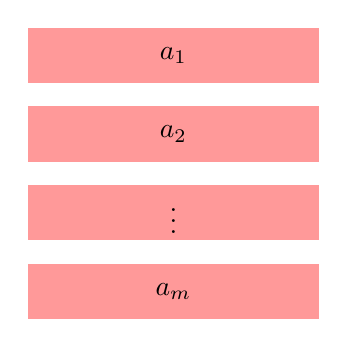
\begin{tikzpicture}
        \pgfmathsetmacro{\elementsize}{0.7}
        \foreach \y in {0, 1, 2, 3}{
                \fill [red, opacity=0.4] ({-1.5-\elementsize/2}, {\y-\elementsize/2}) rectangle ({1.5+\elementsize/2}, {\y+\elementsize/2});
            }
            \node at (0, 3) {$a_1$};
            \node at (0, 2) {$a_2$};
            \node at (0, 1) {$\vdots$};
            \node at (0, 0) {$a_m$};
    \end{tikzpicture}
\end{figure}

我们会发现输出 $y$ 的每一个分量 $y_i$ 都是输入 $x$ 与行 $a_i$ 的点积\footnote{严格地说 $a$ 是行向量,$x$ 是列向量,这中间在数学上有一些差别,是矩阵乘法而不是点积。但是在计算机存储中,因为都是一维数组,从实用的角度并不需要纠结于此,这种\textoverset{Abuse of Notation}{记号混用}就见怪不怪了。}。例如
\[
    y_1 = a_1 \cdot x = a_{11}x_1 + a_{12}x_2 + \cdots + a_{1n}x_n
\]

诚然,每一行都是一个\textoverset{Homogeneous}{齐次的}\footnote{齐次:指不带偏置(常数)项。}线性函数,它的形式也只能是这种 $x$ 的\textoverset{Weighted Sum}{加权和},但是相信一定会有读者好奇:点积衡量了两个向量的相似程度,那么这里做点积的几何意义是什么呢?答曰:探测输入的特征。

我们可以把矩阵的每一行看作一个\textoverset{Feature Detector}{特征检测器},它的方向表明了待检测的特征方向,与 $x$ 的点积则说明了这个输入在这个特征上的响应强度(通常称为\textoverset{Feature Response}{特征响应})。当 $x$ 与特征的方向相近时响应的值为正,而当 $x$ 与特征的方向相反时响应的值会为负,当 $x$ 与特征几乎无关时响应的值会接近于零。这是点积的几何特性,至少从理论上为特征提取画出了一条路径。

这时如果考虑怎么样的输入可以接近预期的输出呢?根据几何解释,其实就是试图找到一个输入向量,让它尽可能通过这些特征检测器,使得每一个特征检测器的响应值与预期的响应(输出的对应分量)尽可能接近,并考虑使用均方误差来“惩罚”不接近的程度,我们一开始的代数解释便是如此。

但是如果改改输出的写法,把矩阵切成若干列,我们又有了一个不同的视角,不过这里我们用 $a_{:j}$ 表示它的列:
\begin{figure}[H]
    \centering
    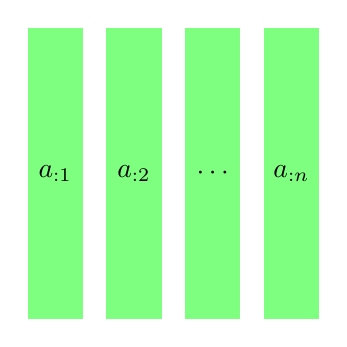
\begin{tikzpicture}
        \pgfmathsetmacro{\elementsize}{0.7}
        \foreach \x in {0, 1, 2, 3}{
                \fill [green, opacity=0.5] ({\x-\elementsize/2}, {-1.5-\elementsize/2}) rectangle ({\x+\elementsize/2}, {1.5+\elementsize/2});
            }
            \node at (0, 0) {$a_{:1}$};
            \node at (1, 0) {$a_{:2}$};
            \node at (2, 0) {$\cdots$};
            \node at (3, 0) {$a_{:n}$};
    \end{tikzpicture}
\end{figure}

这样看来,矩阵的乘法也可以写成
\[
\begin{aligned}
    Ax & = \begin{bmatrix}
        a_{:1} & a_{:2} & \cdots & a_{:n}
    \end{bmatrix}
    \begin{bmatrix}
        x_1 \\ x_2 \\ \vdots \\ x_n
    \end{bmatrix}
    \\
    &= x_1 a_{:1} + x_2 a_{:2} + \cdots + x_n a_{:n}
\end{aligned}
\]

也就是说,输出写成了输入的线性组合。这时我们在输出的空间 $\mathbb{R}^m$ 操作,而输入的空间 $\mathbb{R}^n$ 仅仅是作为权重的载体,给出了这些列向量应该以怎么样的比例组合。

这时我们要怎么考虑用输出反推合适的输入这个问题呢?随着输入的变化,输出会变为列向量的不同组合方式,正如之前所说的,我们需要在这些列向量线性组合形成的超平面上找点,让它和预期的输出尽可能接近,这就是我们在前文提到的最小二乘的几何视角。

最后一种角度则带有更为浓重的\textoverset{Distruction}{解构}\footnote{解构:哲学术语,通常指的是对一个结构或概念进行拆解、分析。}色彩,如果把矩阵看成一个数表,作为一个填了数字的 $m\times n$ 矩形:
\begin{figure}[H]
    \centering
    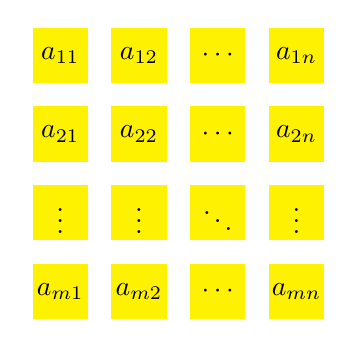
\begin{tikzpicture}
        \pgfmathsetmacro{\elementsize}{0.7}
        \foreach \x in {0, 1, 2, 3}{
                \foreach \y in {0, 1, 2, 3}{
                        \fill [yellow] ({\x-\elementsize/2}, {\y-\elementsize/2}) rectangle ({\x+\elementsize/2}, {\y+\elementsize/2});
                    }
            }
        \node at (0, 3) {$a_{11}$};
        \node at (1, 3) {$a_{12}$};
        \node at (2, 3) {$\cdots$};
        \node at (3, 3) {$a_{1n}$};
        \node at (0, 2) {$a_{21}$};
        \node at (1, 2) {$a_{22}$};
        \node at (2, 2) {$\cdots$};
        \node at (3, 2) {$a_{2n}$};
        \node at (0, 1) {$\vdots$};
        \node at (1, 1) {$\vdots$};
        \node at (2, 1) {$\ddots$};
        \node at (3, 1) {$\vdots$};
        \node at (0, 0) {$a_{m1}$};
        \node at (1, 0) {$a_{m2}$};
        \node at (2, 0) {$\cdots$};
        \node at (3, 0) {$a_{mn}$};
    \end{tikzpicture}
\end{figure}

一般来说,我们的教材都是这么引入的,但是就像我刚才提到的一样,这种理解有着一股解构的色彩。如果没有解构后重新的\textoverset{Construction}{建构}\footnote{建构:哲学术语,通常指的是对一个结构或概念进行重建、整合。},这种理解很容易让人迷失在行列式、特征值、特征向量等等复杂计算的汪洋大海中,从而忘记了矩阵的本质。那么这种解释有什么意义呢?我认为它的作用就在于 $a_{ij}$ 体现了第 $j$ 个输入对第 $i$ 个输出的权重。

让我们看看下面这个示意图:
\begin{figure}[H]
    \centering
    \begin{tikzpicture}[>=Stealth, scale=1.5]
        \pgfmathsetmacro{\elementsize}{0.6}
        \foreach \x in {0, 1, 2, 3}{
                \foreach \y in {0, 1, 2, 3}{
                        \fill [yellow] ({\x-\elementsize/2}, {\y-\elementsize/2}) rectangle ({\x+\elementsize/2}, {\y+\elementsize/2});
                    }
            }
        \foreach \x in {0, 1, 2, 3}{
            \draw [green!80!black, thick] ({\x - 0.2}, 4) -- ({\x - 0.5}, 4) -- ({\x - 0.5}, 0);
            \foreach \y in {0, 1, 2, 3}{
                \draw [->, green!80!black] ({\x - 0.5}, \y) -- ({\x - \elementsize/2}, \y);
            }
        }
        \foreach \y in {0, 1, 2, 3}{
            \draw [red!80!black, thick, ->] (0, {\y + 0.5}) -- (4, {\y + 0.5}) -- (4, {\y + 0.2});
            \foreach \x in {0, 1, 2, 3}{
                \draw [->, red!80!black] (\x, {\y + \elementsize/2}) -- (\x, {\y + 0.5});
            }
        }
        \node at (0, 3) {$a_{11}$};
        \node at (1, 3) {$a_{12}$};
        \node at (2, 3) {$\cdots$};
        \node at (3, 3) {$a_{1n}$};
        \node at (0, 2) {$a_{21}$};
        \node at (1, 2) {$a_{22}$};
        \node at (2, 2) {$\cdots$};
        \node at (3, 2) {$a_{2n}$};
        \node at (0, 1) {$\vdots$};
        \node at (1, 1) {$\vdots$};
        \node at (2, 1) {$\ddots$};
        \node at (3, 1) {$\vdots$};
        \node at (0, 0) {$a_{m1}$};
        \node at (1, 0) {$a_{m2}$};
        \node at (2, 0) {$\cdots$};
        \node at (3, 0) {$a_{mn}$};

        \node at (0, 4) {$x_1$};
        \node at (1, 4) {$x_2$};
        \node at (2, 4) {$\cdots$};
        \node at (3, 4) {$x_n$};

        \node at (4, 3) {$y_1$};
        \node at (4, 2) {$y_2$};
        \node at (4, 1) {$\vdots$};
        \node at (4, 0) {$y_m$};
    \end{tikzpicture}
\end{figure}

矩阵乘法可以看成这样,输入的每个分量沿着列地址线\footnote{地址线:计算机内存中的概念,虽然逻辑上内存是连续的,但是实际上内存寻址时有很多层,最底层时被选择的内存芯片是通过行和列寻址的,物理上由两条地址线输入\textoverset{Row/Column Address Strobe}{行/列地址选通信号。}}输入到每一列的所有块,由每个元素乘上对应的权重后,将结果“上传”到对应的行地址线上,最后在行地址线上的所有块累积起来得到输出的每个分量。

这个图还有另外一个很常见的呈现形式,把它看成一个无偏置的\textoverset{Linear Layer}{线性层}\footnote{线性层:在后面章节的机器学习中会成为一个基本模块,本质上就是从输入 $x$ 得到输出 $y=Ax + b$ 的过程,这里的无偏置即 $b=0$。},我们通常是这样绘制的:
\begin{figure}[H]
    \centering
    \begin{tikzpicture}[>=Stealth, scale=1.5]
        \pgfmathsetmacro{\elementradius}{0.3}
        \foreach \x in {0, 1, 2, 3} {
            \foreach \y in {0, 1, 2, 3} {
                \draw [yellow] (0, \x) -- (5, \y);
            }
        }
        \foreach \x in {0, 1, 2, 3}{
            \fill [green!50!white] (0, \x) circle (\elementradius);
        }
        \foreach \y in {0, 1, 2, 3}{
            \fill [red!50!white] (5, \y) circle (\elementradius);
        }
        \node at (0, 3) {$x_1$};
        \node at (0, 2) {$x_2$};
        \node at (0, 1) {$\vdots$};
        \node at (0, 0) {$x_n$};

        \node at (5, 3) {$y_1$};
        \node at (5, 2) {$y_2$};
        \node at (5, 1) {$\vdots$};
        \node at (5, 0) {$y_m$};

        \node[above] at (2.5, 3) {$a_{11}$};
        \foreach \y in {0.5, 1.0, ..., 2.5}{
        \node at (2.5, \y) {$\vdots$};}
        \node[below] at (2.5, 0) {$a_{mn}$};
    \end{tikzpicture}
\end{figure}

每条从 $x$ 到 $y$ 的连线都代表有一个从 $x$ 到 $y$ 的权重,我们给 $x_j$ 到 $y_i$ 的连线赋予权重 $a_{ij}$,它就表明了输入 $x_j$ 是如何影响输出 $y_i$ 的。

至此我们已经从四个有差别但是又有联系的视角理解了矩阵的行为,不过我觉得我对于不同的解释还有一点观察。当降维时,特征提取(行的视角)体现的更明显,而当升维时,特征组合(列的视角)更为重要。降维伴随着对信息的压缩和精简,通过去掉不重要的部分,更接近事物的本质。升维不仅仅是增加维度,更是通过新的空间来赋予数据提供更多的可变性。在这个过程中,每一列代表了一个基向量,整个矩阵的列向量按比例组合出高维的结果。

花了一些篇幅来复习线性代数,是时候回到多元线性拟合的问题上了。不过这次可以使用矩阵的语言来描述这个问题了。假设我们有 $n$ 组 $d$ 维的 $x$ 的取值,它们组成了一个 $n\times d$ 的矩阵 $\bfx$\,\footnote{记号说明:使用大写字母表示矩阵的比较多,但是这里为了美观和符号的一致性,我们仍然采用黑体小写字母表示所有数据点的集合。$\bfx_i$ 表示第 $i$ 个数据点,$\bfx_{:j}$ 表示所有数据点的第 $j$ 个分量,$x_{ij}$ 表示第 $i$ 个数据点的第 $j$ 个分量,因为是标量,所以采取小写。而在方程 $x\cdot w$ 中,$x,w$ 并非数据点的集合,而是变量,故虽然为向量,但是采用斜体。}。我们的目标是找到一个 $d$ 维的 $w$,使得数据集上 $x\cdot w$ 尽可能接近 $y$,现在 $\hat y$ 的表达式用点积的语言可以简洁地写为 $\hat y = x\cdot w + b$ 这种形式。

但是通过一点点技巧可以让问题更简洁,在拟合函数中,我们可以把 $b$ 合并到 $w$ 中,也就是
\[
\begin{aligned}
    \hat y &= x \cdot w + b \\
    &= x_1 w_1 + x_2 w_2 + \cdots + x_d w_d + b\\
    &= \begin{bmatrix}
        x_{1} & x_{2} & \cdots & x_{d} & 1
    \end{bmatrix}
    \begin{bmatrix}
        w_1 \\ w_2 \\ \vdots \\ w_d \\ b
    \end{bmatrix}
\end{aligned}
\]

对于样本,把所有的行并起来就变成了不需要额外添加偏置的 $\hat \bfy = \tilde \bfx \tilde w$。如果要说这个 $\tilde \bfx$ 是什么,它就是把 $\bfx$ 的每一行拼上一个 $1$:
\begin{figure}[H]
    \centering
    \begin{tikzpicture}
        \pgfmathsetmacro{\elementsize}{0.7}
        \fill [gray, opacity=0.5] ({-2-\elementsize/2}, {-\elementsize/2}) rectangle ({-2+\elementsize/2}, {3+\elementsize/2});
        \node at (-2, 1.5) {$\hat \bfy$};
        \draw ({-2-\elementsize/2}, -0.5) -- (-2.5, -0.5) -- (-2.5, 3.5) -- ({-2-\elementsize/2}, 3.5);
        \draw ({-2+\elementsize/2}, -0.5) -- (-1.5, -0.5) -- (-1.5, 3.5) -- ({-2+\elementsize/2}, 3.5);
        \node at (-1, 1.5) {$=$};
        \foreach \y in {0, 1, 2, 3}{
                \fill [red, opacity=0.4] ({0-\elementsize/2}, {\y-\elementsize/2}) rectangle ({2+\elementsize/2}, {\y+\elementsize/2});
            }
            \node at (1, 3) {$\bfx_1$};
            \node at (1, 2) {$\bfx_2$};
            \node at (1, 1) {$\vdots$};
            \node at (1, 0) {$\bfx_n$};
        \fill [green, opacity=0.5] ({3-\elementsize/2}, {-\elementsize/2}) rectangle ({3+\elementsize/2}, {3+\elementsize/2});
        \node at (3, 1.5) {$1$};
        \draw ({-\elementsize/2}, -0.5) -- (-0.5, -0.5) -- (-0.5, 3.5) -- ({-\elementsize/2}, 3.5);
        \draw ({3+\elementsize/2}, -0.5) -- (3.5, -0.5) -- (3.5, 3.5) -- ({3+\elementsize/2}, 3.5);
        \fill [red, opacity=0.4] ({5-\elementsize/2}, {1-\elementsize/2}) rectangle ({5+\elementsize/2}, {3+\elementsize/2});
        \fill (4, 1.5) circle (0.05);
        \node at (5, 2) {$w$};
        \fill [green, opacity=0.5] ({5-\elementsize/2}, {-\elementsize/2}) rectangle ({5+\elementsize/2}, {0+\elementsize/2});
        \node at (5, 0) {$b$};
        \draw ({5-\elementsize/2}, -0.5) -- (4.5, -0.5) -- (4.5, 3.5) -- ({5-\elementsize/2}, 3.5);
        \draw ({5+\elementsize/2}, -0.5) -- (5.5, -0.5) -- (5.5, 3.5) -- ({5+\elementsize/2}, 3.5);
    \end{tikzpicture}
\end{figure}

但是如果改成用列的视角来看待矩阵 $\tilde \bfx$,我们会发现问题变成了用 $\bfx_{:1}, \bfx_{:2}, \cdots, \bfx_{:d}$ 与 $\bfx^0$ 的线性组合来贴近 $\bfy$。
\begin{figure}[H]
    \centering
    \begin{tikzpicture}
        \pgfmathsetmacro{\elementsize}{0.7}
        \fill [gray, opacity=0.5] ({-2-\elementsize/2}, {-\elementsize/2}) rectangle ({-2+\elementsize/2}, {3+\elementsize/2});
        \node at (-2, 1.5) {$\hat \bfy$};
        \draw ({-2-\elementsize/2}, -0.5) -- (-2.5, -0.5) -- (-2.5, 3.5) -- ({-2-\elementsize/2}, 3.5);
        \draw ({-2+\elementsize/2}, -0.5) -- (-1.5, -0.5) -- (-1.5, 3.5) -- ({-2+\elementsize/2}, 3.5);
        \node at (-1, 1.5) {$=$};
        \foreach \x in {0, 1, 2}{
                \fill [green, opacity=0.5] ({\x-\elementsize/2}, {0-\elementsize/2}) rectangle ({\x+\elementsize/2}, {3+\elementsize/2});
            }
            \node at (0, 1.5) {$\bfx_{:1}$};
            \node at (1, 1.5) {$\cdots$};
            \node at (2, 1.5) {$\bfx_{:d}$};
        \fill [green, opacity=0.5] ({3-\elementsize/2}, {-\elementsize/2}) rectangle ({3+\elementsize/2}, {3+\elementsize/2});
        \node at (3, 1.5) {$1$};
        \draw ({-\elementsize/2}, -0.5) -- (-0.5, -0.5) -- (-0.5, 3.5) -- ({-\elementsize/2}, 3.5);
        \draw ({3+\elementsize/2}, -0.5) -- (3.5, -0.5) -- (3.5, 3.5) -- ({3+\elementsize/2}, 3.5);
        \foreach \y in {0, 1, 2, 3}{
                \fill [yellow] ({5-\elementsize/2}, {\y-\elementsize/2}) rectangle ({5+\elementsize/2}, {\y+\elementsize/2});
            }
            \node at (5, 3) {$w_1$};
            \node at (5, 2) {$\vdots$};
            \node at (5, 1) {$w_d$};
            \node at (5, 0) {$b$};
        \fill (4, 1.5) circle (0.05);
        \node at (5, 0) {$b$};
        \draw ({5-\elementsize/2}, -0.5) -- (4.5, -0.5) -- (4.5, 3.5) -- ({5-\elementsize/2}, 3.5);
        \draw ({5+\elementsize/2}, -0.5) -- (5.5, -0.5) -- (5.5, 3.5) -- ({5+\elementsize/2}, 3.5);
    \end{tikzpicture}
\end{figure}

诶?这不是函数拟合问题吗?如果把 $\bfy$ 和 $\bfx_{:j}$ 看作是关于 $i$ 的函数(这里函数定义在 $\{1, 2, \cdots, n\}$ 上,换言之,记 $\bfy(1) = y_1, \bfy(2) = y_2, \cdots, \bfy(n) = y_n$,同理,设 $\bfx_{:j}(i) = x_{ij}$。那么我们的问题就是用 $d$ 个函数 $\bfx_{:1}(i) \sim \bfx_{:d}(i)$ 与一个常值函数 $\bfx^{0}(i) \equiv 1$ 来拟合一个给定的函数 $\bfy(i)$。

去掉常数项(或者把常数项也当成一个 $\bfx_{:d+1}$ )并把自变量 $i$ 当成一元函数拟合问题中的 $x$ 就可以发现:这与使用给定函数 $f_1(x)\sim f_d(x)$ 的线性组合,在若干数据点上拟合给定函数 $f(x)$ 这一问题没有任何差别。由此可见,用给定的函数集来拟合一个函数本质上与多元线性拟合有着完全相同的数学结构。

至此,我们至少已经初步理解了线性拟合。在这一章的最后,让我们做个总结。

\begin{itemize}
    \item 最开始我们引入了一元的线性拟合,学会了最小二乘法与最小化损失以优化参数的基本思想,也学会了如何给数据加权。
    \item 接下来来到了多项式拟合,虽然是曲线,但是如果把 $x$ 的方幂看作线性独立的分量,这仍然可以看作是一种线性拟合,在这里我们领略到了过拟合的危害,也理解了为什么要使用正则化与归一化方法。
    \item 在过拟合中,我们得到的更重要的启示是要意识到高次并不意味着万能,合适的才是最好。如果参数足以存下所有的数据,那么大概率就会过拟合。
    \item 最后我们引入了多元线性拟合,通过矩阵的不同解读,我们理解了特征提取与特征重组的逻辑。
    \item 从矩阵的行、列解读中,我们意识到多元线性拟合与函数的线性拟合本质上是一样的,这里有一种精妙的对应关系。
\end{itemize}

\begin{tcolorbox}[myrecommendbox, title=推荐阅读, breakable=false]
    \begin{itemize}
        \item The Art of Linear Algebra 这篇文章非常好,但是如果你上不去 GitHub,进这个知乎回答看也行:\\
              \textit{如何快速理解线性代数? - 丿小奇迹丨的回答 - 知乎}\\
              \url{https://www.zhihu.com/question/30726396/answer/3124578647}
            \item 这篇文章推荐给数理统计与线性代数都学的较好的读者:\\
                  \textit{回归分析|笔记整理(6)——多元线性回归(上) - 学弱猹的文章 - 知乎}\\
                  \url{https://zhuanlan.zhihu.com/p/48541799}
    \end{itemize}
\end{tcolorbox}